
\section{ОГЛЯД ТА ВИБІР ТЕХНОЛОГІЙ ДЛЯ ПРОЕКТУВАННЯ СИСТЕМИ}

\subsection{Загальні принципи побудови кросплатформних мобільних застосунків}

\subsubsection{Клієнт-серверна архітектура мобільних застосунків}

Більшість сучасних мобільних застосунків побудовано за клієнт-серверною архітектурою: клієнтська частина (мобільний застосунок) відповідає за відображення даних і взаємодію з користувачем, тоді як серверна частина забезпечує зберігання, обробку та ізоляцію даних. Такий поділ дозволяє масштабувати компоненти системи незалежно: бекенд може обслуговувати одночасно iOS- та Android-клієнтів без дублювання бізнес-логіки.

У контексті розроблення мобільних клієнтів виокремлюють три основні підходи, що відрізняються балансом між продуктивністю, витратами на розробку та доступом до платформних можливостей.

Нативна розробка передбачає окремі кодові бази для iOS (Swift/Objective-C) та Android (Kotlin/Java). Цей підхід забезпечує найвищу продуктивність, повний доступ до платформних \gls{API} та найкраще відчуття платформи, однак вимагає підтримки двох незалежних кодових баз, що подвоює витрати на розробку та тестування.

Гібридний підхід базується на вебтехнологіях (HTML/CSS/JavaScript), загорнутих у нативну оболонку за допомогою таких фреймворків, як Ionic або Capacitor. Спільна кодова база суттєво знижує витрати, проте застосунок виконується у WebView, що призводить до помітних затримок при рендерингу та нестандартної поведінки нативних елементів \gls{UI}.

Кросплатформна нативна розробка поєднує переваги обох підходів: єдина кодова база транспілюється або компілюється у нативний код для кожної платформи. Серед представників цього підходу виокремлюють React Native від Meta та Flutter від Google. React Native відображає компоненти через нативний міст платформи, тоді як Flutter використовує власний рушій рендерингу Skia/Impeller. Обидва інструменти дозволяють досягти продуктивності, близької до нативної, при значно менших витратах на розробку.

Для розроблюваного застосунку обрано кросплатформну нативну розробку на базі React Native. Ключовими факторами вибору є зрілість екосистеми JavaScript/TypeScript, пряма інтеграція з Supabase \gls{SDK} та Expo, а також можливість повторного використання вебкомпонентів. На відміну від Flutter, React Native не потребує вивчення мови Dart і органічно вписується в існуючу екосистему npm-пакетів.

\subsubsection{Основні компоненти мобільного застосунку}

Архітектура розроблюваного застосунку організована у чотири логічних шари з односпрямованою залежністю: вищий шар може звертатись до нижчого, але не навпаки, що запобігає циклічним залежностям і спрощує тестування.

Найближчим до користувача є шар представлення (\textit{Presentation layer}), що містить компоненти \gls{UI}, екрани та навігаційну структуру. У застосунку він реалізований на базі Expo Router із файловою маршрутизацією: кожен файл у директорії \texttt{app/} автоматично відповідає окремому маршруту, а вкладеність директорій визначає ієрархію навігації. Компоненти цього шару отримують дані виключно через пропси або React-хуки і ніколи не звертаються до \gls{API} напряму.

Під ним розташований шар бізнес-логіки (\textit{Business logic layer}), відповідальний за трансформацію даних, валідацію та управління станом застосунку. Він реалізований через кастомні React-хуки та глобальне сховище Zustand, у якому зберігаються поточний профіль дитини і стан автентифікаційної сесії. Цей шар виступає посередником між представленням і даними: він формує запити до \gls{API} та передає готові до відображення об'єкти вгору по стеку.

Шар даних (\textit{Data layer}) забезпечує взаємодію з хмарним \gls{API} та управління локальним кешем. Він реалізований через клієнт Supabase у поєднанні з TanStack Query, що автоматично кешує відповіді сервера, виконує фонове оновлення при поверненні застосунку на передній план і повторює невдалі запити після відновлення мережевого з'єднання.

Основу стеку складає хмарний бекенд (\textit{Backend layer}) --- PostgreSQL з увімкненим \gls{RLS}, автентифікаційний сервіс Supabase Auth, Realtime-підписки для синхронізації між пристроями. Бекенд не передбачає окремого серверного застосунку: бізнес-правила інкапсульовано безпосередньо у \gls{SQL}-функції та тригери бази даних, що скорочує кількість рухомих частин системи.

Взаємодію між шарами схематично зображено на рис.~\ref{fig:architecture}: кожен вищий шар залежить від нижчого, але не навпаки, що унеможливлює циклічні залежності.

\begin{figure}[H]
\centering
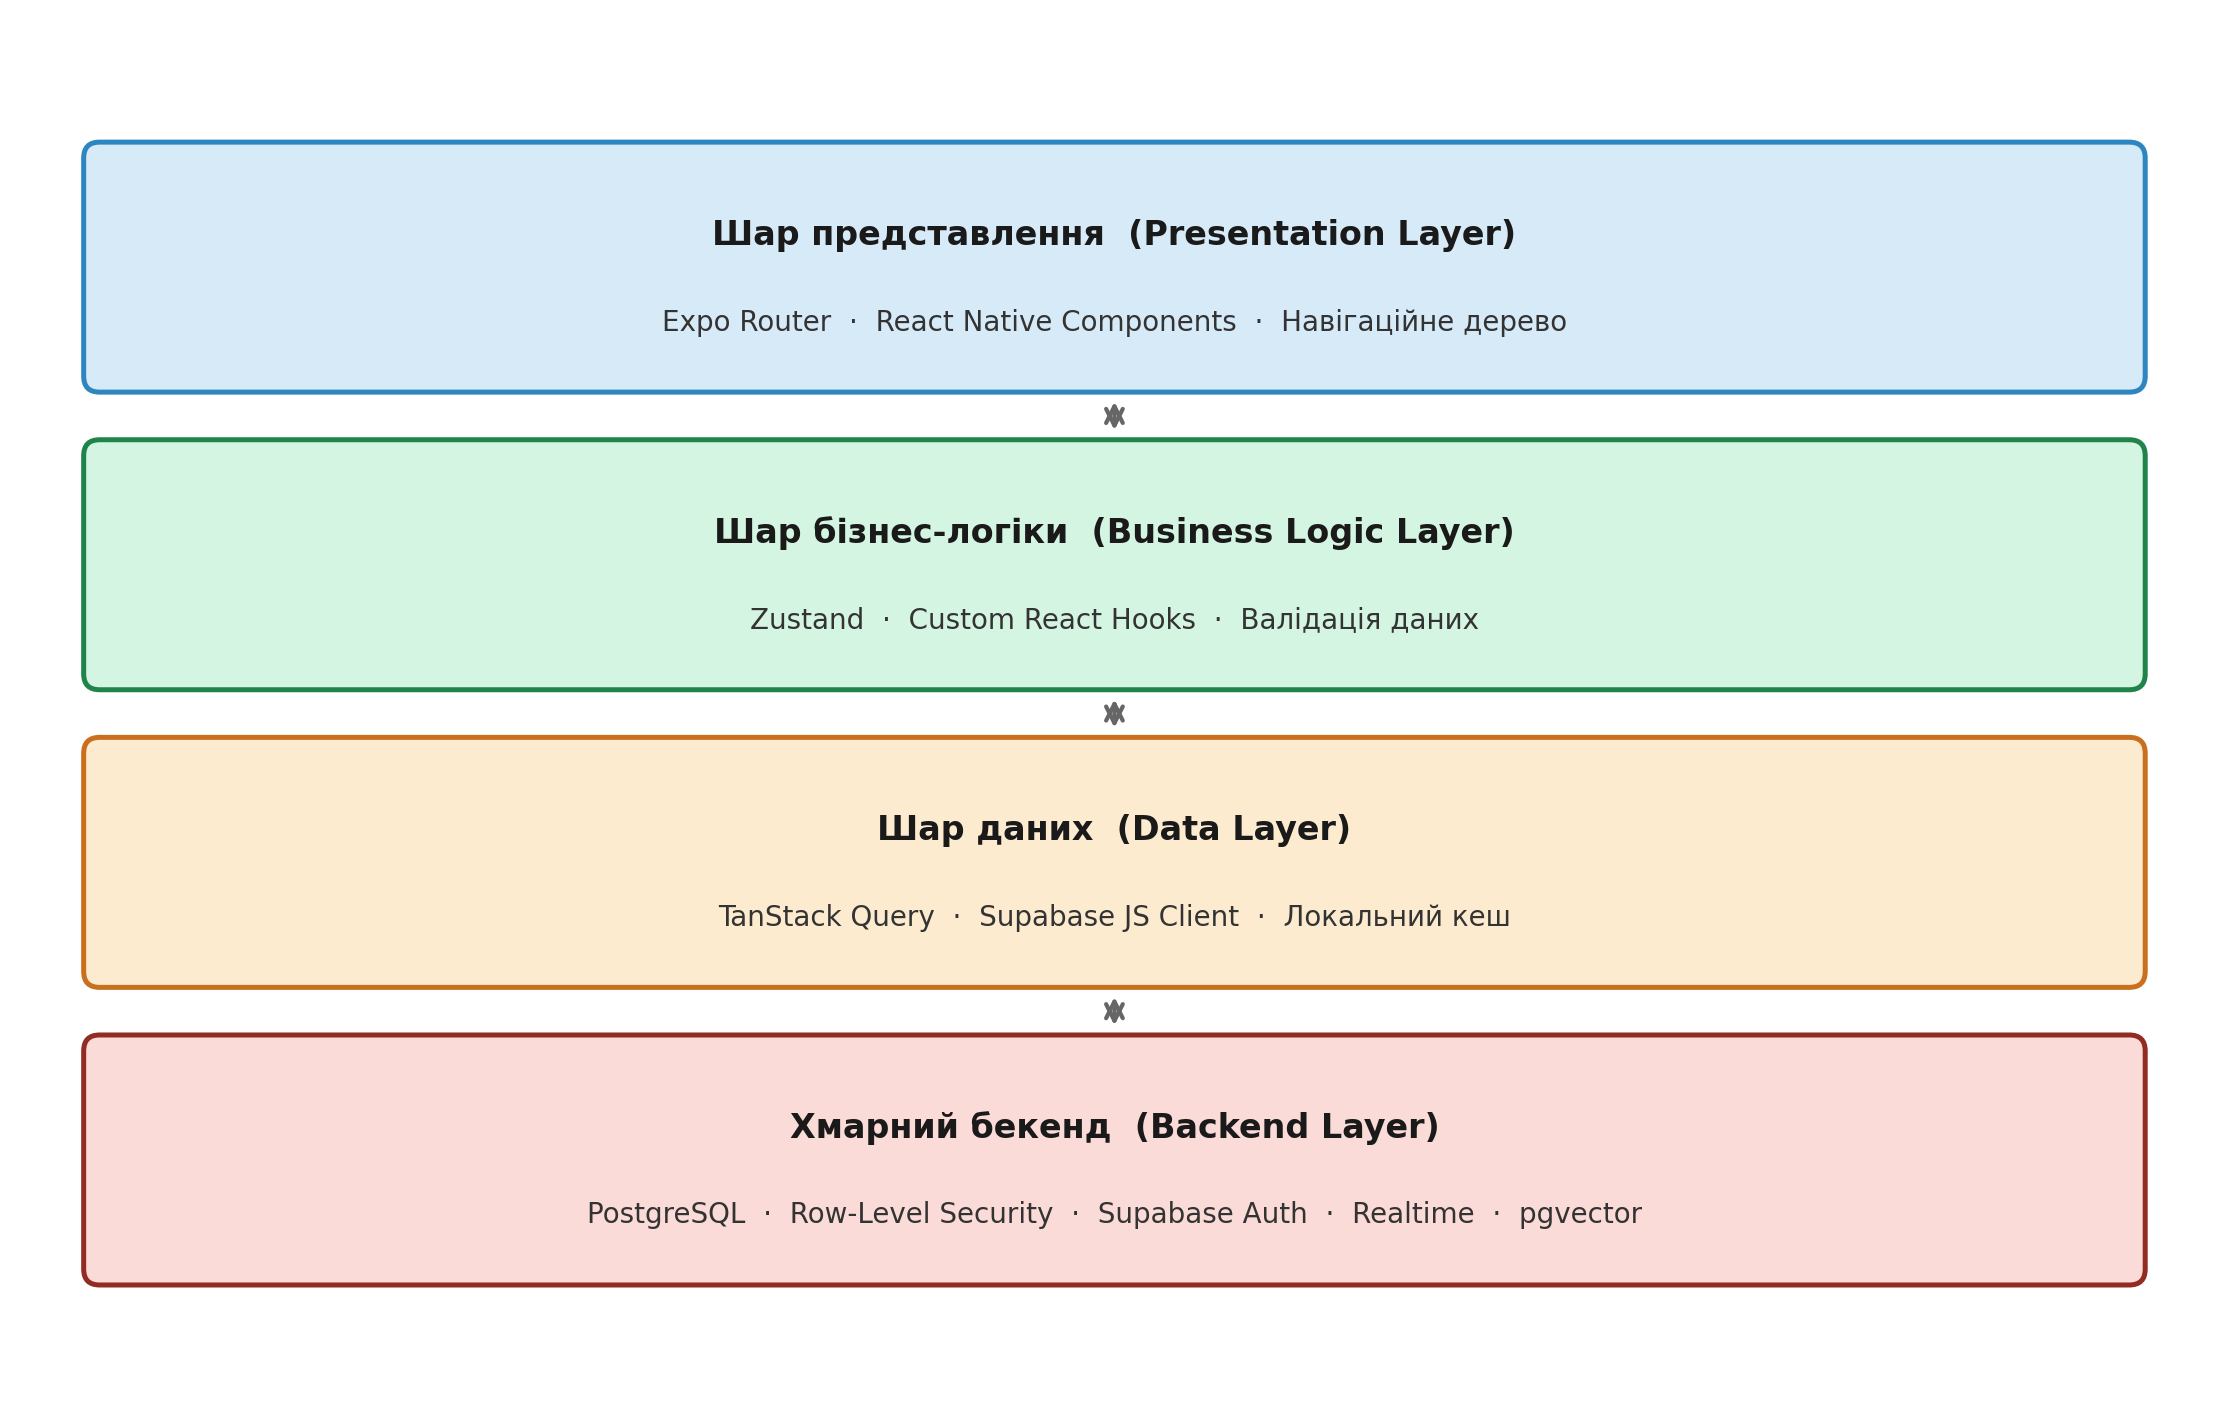
\includegraphics[width=0.95\textwidth]{figures/architecture}
\caption{Чотиришарова архітектура мобільного застосунку}
\label{fig:architecture}
\end{figure}

\subsection{Огляд технологій для реалізації застосунку}

\subsubsection{Технології клієнтської частини}

React Native --- фреймворк від компанії Meta для розроблення нативних мобільних застосунків із використанням JavaScript та TypeScript. На відміну від гібридних рішень, компоненти React Native транслюються безпосередньо у нативні елементи \gls{UI} кожної платформи без проміжного WebView, що забезпечує продуктивність, порівнянну з нативними застосунками. Єдина кодова база для iOS та Android у поєднанні з великою екосистемою npm-пакетів і підтримкою гарячого оновлення (Fast Refresh) суттєво прискорює цикл розробки.

Expo є офіційно рекомендованою надбудовою над React Native, що надає уніфікований \gls{SDK} для доступу до нативних можливостей пристрою (камера, сповіщення, сенсори) без необхідності писати нативний код на Swift чи Kotlin. На відміну від bare React Native, Expo керує конфігурацією нативних проєктів автоматично через систему плагінів, що спрощує обслуговування і оновлення залежностей. Expo Router реалізує файлову маршрутизацію за аналогією з Next.js: структура директорій \texttt{app/} безпосередньо визначає навігаційне дерево застосунку, усуваючи потребу в ручному описі маршрутів.

\subsubsection{Хмарна платформа та серверна частина}

Supabase --- відкрита альтернатива Firebase на базі PostgreSQL. Платформа надає такі сервіси:
\begin{itemize}
  \item реляційна база даних PostgreSQL з повноцінною підтримкою \gls{SQL};
  \item автентифікація (email/пароль, OAuth, magic link);
  \item \gls{REST} та GraphQL \gls{API}, автоматично згенеровані з схеми \gls{БД};
  \item Realtime --- двостороння синхронізація змін у таблицях через WebSocket;
  \item Storage --- зберігання файлів і зображень;
\end{itemize}

Supabase розгорнуто на хмарній інфраструктурі AWS і масштабується автоматично. Вибір Supabase замість Firebase обумовлений повноцінною підтримкою реляційних запитів, відкритим вихідним кодом та можливістю самостійного розгортання.

\subsubsection{Характеристика системи управління базами даних}

PostgreSQL --- потужна об'єктно-реляційна \gls{СУБД} з відкритим вихідним кодом. У контексті розроблюваної системи PostgreSQL відіграє центральну роль: зберігає всі медико-біологічні дані, забезпечує транзакційну цілісність і реалізує \gls{RLS}.

\subsubsection{Управління станом, локалізація та допоміжні бібліотеки}

TanStack Query реалізує декларативне управління асинхронним станом: кешування, фонове оновлення, повторні спроби та синхронізацію запитів між компонентами. Бібліотека суттєво спрощує взаємодію клієнта з \gls{API} та усуває потребу в ручному управлінні станами завантаження й помилок.

Zustand --- мінімалістична бібліотека глобального стану для React та React Native. На відміну від Redux, вона не вимагає шаблонного коду і надає простий \gls{API} для створення сховищ. У розроблюваному застосунку Zustand використовується для зберігання поточного профілю дитини та налаштувань сесії.

i18next --- фреймворк інтернаціоналізації для JavaScript, що забезпечує підтримку декількох мов у застосунку. Застосунок підтримує українську та англійську локалізацію з автоматичним визначенням мови пристрою та можливістю ручного перемикання.

react-native-gifted-charts --- бібліотека графіків для React Native, що використовується для відображення антропометричних даних дитини та стандартних кривих \gls{ВООЗ}. Бібліотека надає гнучкий \gls{API} для побудови лінійних і комбінованих графіків безпосередньо на нативному Canvas.

\subsection{Механізми автентифікації та захисту даних}

Безпека медико-біологічних даних дитини є критичною вимогою системи. Розроблювана архітектура реалізує захист на двох незалежних рівнях: на рівні транспорту всі запити передаються виключно через \gls{HTTPS}, а на рівні \gls{СУБД} доступ до рядків таблиць обмежується механізмом \gls{RLS}.

Автентифікація здійснюється через Supabase Auth, що видає підписаний \gls{JWT}-токен після успішного входу. Цей токен передається в заголовку кожного \gls{API}-запиту та використовується \gls{СУБД} для визначення поточного користувача.

\subsubsection{Row-Level Security та ізоляція даних користувачів}

\gls{RLS} --- механізм PostgreSQL, що дозволяє визначати умови видимості рядків таблиці на рівні \gls{СУБД}. При увімкнутому \gls{RLS} кожен \gls{SQL}-запит автоматично отримує додаткові умови фільтрації, визначені відповідними політиками безпеки.

У розроблюваній системі кожна таблиця (профілі дітей, активності, вимірювання, вакцинації) має набір \gls{RLS}-політик, що дозволяють користувачу читати та змінювати лише власні записи. Ідентифікатор користувача витягується безпосередньо з \gls{JWT}-токена функцією \texttt{auth.uid()}, що унеможливлює підробку ідентичності навіть за наявності прямого доступу до \gls{API}.

Таким чином, \gls{RLS} надає додатковий рівень захисту, незалежний від логіки застосунку: навіть якщо клієнтський код містить помилку авторизації, \gls{СУБД} не поверне чужих даних.

\subsubsection{Безпека мобільного застосунку}

Мобільний застосунок, що обробляє персональні медичні дані, є потенційною ціллю для реверс-інжинірингу та несанкціонованого доступу. Для захисту на рівні клієнтського середовища виконання інтегровано два інструменти.

freeRASP --- бібліотека захисту мобільного застосунку в режимі виконання (\textit{Runtime Application Self-Protection}). Вона виявляє загрозливе середовище: root-доступ або jailbreak на пристрої, підключені дебагери, запуск у емуляторі, а також ознаки переупакування або підробки застосунку. У разі виявлення загрози застосунок може заблокувати виконання критичних операцій або завершити сесію.

Sentry --- платформа моніторингу помилок і продуктивності. Інтеграція Sentry дозволяє в реальному часі отримувати звіти про необроблені винятки, падіння застосунку та повільні мережеві запити. Це суттєво скорочує час виявлення та виправлення дефектів у виробничому середовищі.

\subsection{Стандарти ВООЗ та педіатричний моніторинг}

\gls{ВООЗ} у 2006 році опублікувала Стандарти зростання дитини (\textit{Child Growth Standards}) --- набір перцентильних кривих, що описують нормальний фізичний розвиток дітей від народження до п'яти років. Стандарти побудовані на основі міжнародного мультицентрового дослідження за участю дітей із шести країн і вважаються глобальним еталоном.

Для кожного показника (маса тіла, зріст, окружність голови) та кожної статі визначено п'ять перцентильних ліній: P3, P15, P50, P85 та P97. Значення P50 відповідає медіані популяції, P3 --- нижній межі норми, P97 --- верхній. Відхилення вимірювання за межі P3 або P97 є підставою для консультації з педіатром.

У розроблюваному застосунку перцентильні таблиці \gls{ВООЗ} вбудовано статично для діапазону 0--24 місяці окремо для хлопчиків і дівчаток. При додаванні нового вимірювання застосунок автоматично визначає перцентиль дитини і відображає її положення на графіку відносно кривих норми. Статичне вбудовування таблиць усуває залежність від мережевого підключення при перегляді антропометричних даних.

\subsection{Ключові алгоритми обробки медико-біологічних даних}

\subsubsection{Алгоритм ШІ-асистента на основі RAG}

ШІ-асистент реалізує педіатричні консультації на основі технології Retrieval-Augmented Generation (\gls{RAG}) --- підходу, що поєднує векторний пошук у базі знань із генеративною мовною моделлю. На відміну від чистої генерації, \gls{RAG} обмежує відповіді контекстом верифікованих педіатричних документів, що суттєво знижує ризик галюцинацій та невірних медичних рекомендацій.

Алгоритм складається з п'яти послідовних кроків, схему яких наведено на рис.~\ref{fig:rag-pipeline}.

На першому кроці запит користувача перетворюється на числовий вектор (embedding) за допомогою моделі nomic-embed-text. Цей вектор кодує семантичний зміст запиту у просторі фіксованої розмірності та є основою для подальшого пошуку.

На другому кроці вектор запиту використовується для пошуку найближчих сусідів у сховищі векторних embedding педіатричної бази знань, що зберігаються у розширенні pgvector бази даних PostgreSQL. Пошук виконується за косинусною подібністю та повертає п'ять найбільш релевантних фрагментів.

Отримані фрагменти формують \gls{RAG}-контекст, що поєднується із системним промптом. Системний промпт визначає роль асистента, мову відповіді та обмеження компетенції.

Сформований промпт передається до Groq \gls{API} --- сервісу швидкого виведення великих мовних моделей (\gls{LLM}) на апаратному прискорювачі LPU. Groq забезпечує швидкість генерації до 500~токенів/с, що дозволяє реалізувати стрімінгові відповіді без помітних затримок. Відповідь \gls{LLM} повертається клієнту через потоковий Supabase Edge Function і відображається у чаті в режимі реального часу.

Детальна реалізація серверної функції та логіки запитів розглянута у підрозділі~3.2.

\begin{figure}[H]
\centering
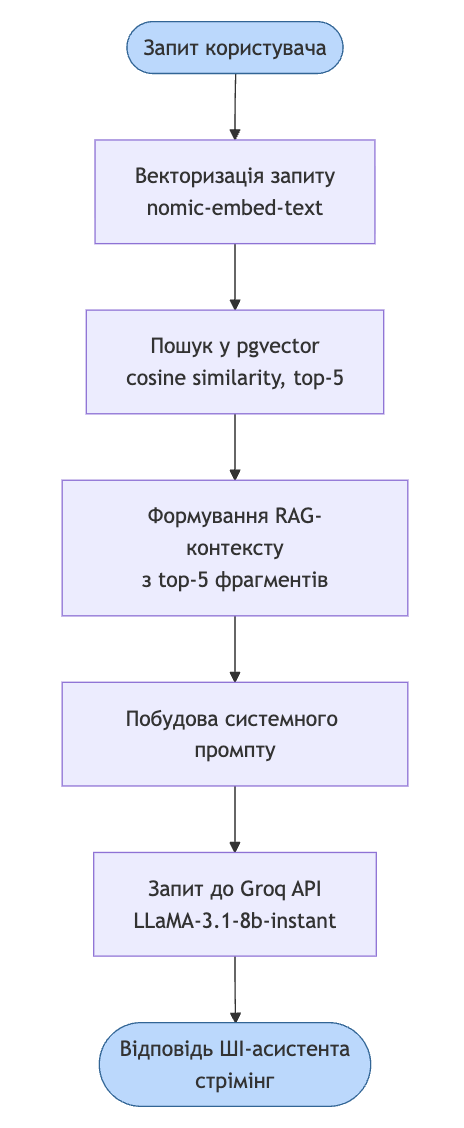
\includegraphics[width=0.44\textwidth]{figures/rag-pipeline}
\caption{Схема алгоритму роботи ШІ-асистента на основі RAG}
\label{fig:rag-pipeline}
\end{figure}

\subsubsection{Алгоритм перцентильної класифікації антропометричних показників}

Для оцінювання фізичного розвитку дитини застосунок реалізує алгоритм класифікації антропометричних показників на основі перцентильних таблиць \gls{ВООЗ}. Алгоритм приймає на вхід значення показника (маса тіла, зріст або окружність голови), вік дитини в місяцях та стать, а повертає перцентильну зону та інтерпольовані значення ліній P3, P15, P50, P85, P97.

Ключовим кроком є лінійна інтерполяція між двома суміжними рядками таблиці для точного обчислення перцентилів при довільному віці. Результат класифікації визначає одну з п'яти зон: нижче P3, P3--P15, P15--P85 (норма), P85--P97 або вище P97. Відхилення за межі P3 або P97 є підставою для консультації з педіатром.

Перцентильні таблиці \gls{ВООЗ} вбудовано статично у застосунок для діапазону 0--24~місяці окремо для хлопчиків і дівчаток, що усуває залежність від мережевого підключення. Принципову схему алгоритму наведено у додатку~А.

\begin{unnumbered}

\section{ВИСНОВОК ДО РОЗДІЛУ 2}

У другому розділі визначено технологічний стек та архітектурні принципи розроблюваної системи. Обґрунтовано вибір клієнт-серверної архітектури з чотирма логічними шарами: представлення, бізнес-логіки, даних і хмарного бекенду. Показано, що кросплатформна нативна розробка є оптимальним підходом для охоплення iOS та Android при єдиній кодовій базі.

Обрано React Native та Expo як основу клієнтської частини. React Native забезпечує нативне відображення компонентів без WebView, а Expo спрощує доступ до платформних можливостей і управління конфігурацією нативних проєктів через систему плагінів.

Хмарну платформу Supabase на базі PostgreSQL обрано завдяки підтримці реляційних запитів, механізму \gls{RLS} для ізоляції даних між користувачами та вбудованому сервісу синхронізації в реальному часі.

Для управління станом обрано TanStack Query --- для асинхронних запитів з автоматичним кешуванням, та Zustand --- для глобального стану застосунку. Локалізацію забезпечує i18next з підтримкою української та англійської мов, а react-native-gifted-charts використовується для побудови антропометричних графіків із кривими \gls{ВООЗ}. Захист виконуваного середовища реалізовано через freeRASP, моніторинг помилок --- через Sentry.

Розглянуто стандарти \gls{ВООЗ} щодо фізичного розвитку дітей і спосіб їх статичної інтеграції у застосунок у вигляді перцентильних таблиць для діапазону 0--24~місяці.

Описано ключові алгоритми системи: алгоритм ШІ-асистента на основі \gls{RAG} з використанням nomic-embed-text, pgvector та Groq \gls{API}, а також алгоритм перцентильної класифікації антропометричних показників за стандартами \gls{ВООЗ}. Реалізацію цих алгоритмів розглянуто у третьому розділі.

\end{unnumbered}
